\documentclass[t]{beamer}  % [t], [c], или [b] --- вертикальное выравнивание на слайдах (верх, центр, низ)

% \documentclass[t]{beamer}  % [t], [c], или [b] --- вертикальное выравнивание на слайдах (верх, центр, низ)
%\documentclass[handout]{beamer} % Раздаточный материал (на слайдах всё сразу)
%\documentclass[aspectratio=169]{beamer} % Соотношение сторон

\usetheme{Berlin} % Тема оформления
%\usetheme{Madrid}
%\usetheme{Frankfurt}
%\usetheme{CambridgeUS}

\usecolortheme{albatross} % Цветовая схема
%\usecolortheme{monarca} % Цветовая схема
%\usecolortheme{fly} % Цветовая схема
%\useinnertheme{circles}
%\useinnertheme{rectangles}

%\usetheme{HSE}

%%% Работа с русским языком
\usepackage{cmap}					% поиск в PDF
\usepackage{mathtext} 				% русские буквы в формулах
\usepackage[T2A]{fontenc}			% кодировка
% \usepackage[utf8]{inputenc}			% кодировка исходного текста
\usepackage[english,ukrainian]{babel}	% локализация и переносы
\usepackage{amsmath}
\usepackage{amsfonts}
\usepackage{amssymb}

\usepackage{hyperref}

%%% Работа с картинками
\usepackage{graphicx}  % Для вставки рисунков
\graphicspath{{images/}{images2/}}  % папки с картинками
\setlength\fboxsep{3pt} % Отступ рамки \fbox{} от рисунка
\setlength\fboxrule{1pt} % Толщина линий рамки \fbox{}
\usepackage{wrapfig} % Обтекание рисунков текстом

%%% Работа с таблицами
\usepackage{array,tabularx,tabulary,booktabs} % Дополнительная работа с таблицами
\usepackage{longtable}  % Длинные таблицы
\usepackage{multirow} % Слияние строк в таблице

%%% Программирование
\usepackage{etoolbox} % логические операторы

%%% Другие пакеты
\usepackage{lastpage} % Узнать, сколько всего страниц в документе.
\usepackage{soul} % Модификаторы начертания
\usepackage{csquotes} % Еще инструменты для ссылок
%\usepackage[style=authoryear,maxcitenames=2,backend=biber,sorting=nty]{biblatex}
\usepackage{multicol} % Несколько колонок

%%% Картинки
\usepackage{tikz} % Работа с графикой
\usepackage{pgfplots}
\usepackage{pgfplotstable}

\title[Python]{Мова програмування Python для початківців}
%\subtitle{За матеріалами "Системне адміністрування Linux" Сергія Клочкова}
\author{Легенький М.М.}
\date{\today}
\institute[Факультет радіофізики, біомедичної електроніки та комп'ютерних систем]{Факультет радіофізики, біомедичної електроніки та комп'ютерних систем}

\setbeamertemplate{caption}[numbered]

\titlegraphic { 
\begin{tikzpicture}[overlay,remember picture]
\node[left=0.2cm] at (current page.32){
    
\includegraphics[width=3cm]{rbecs_logo}
};
\node[right=0cm] at (current page.148){
    
\includegraphics[width=1.5cm]{python_logo}
};
\end{tikzpicture}
}

\logo{
\begin{tikzpicture}[overlay,remember picture]
\node[left=0cm] at (current page.-26){
    
\includegraphics[width=3cm]{rbecs_logo}
};
\node[right=0cm] at (current page.-153){
    
\includegraphics[width=1.5cm]{python_logo}
};
\end{tikzpicture}}


% \includeonly{presentaion2} 
%\includeonly{file2,file3} % пробела после запятой быть не должно

\begin{document}

\frame[plain]{\titlepage}	% Титульный слайд

\begin{frame}{План лекції}
    \tableofcontents
\end{frame}

% \section*{Лекція 1: Знайомство з Python}
 
\subsection{Вступ}
\begin{frame}
\frametitle{Викладач}
\begin{wrapfigure}{r}{0.35\textwidth}

\includegraphics[width=0.25\textwidth]{pictures/myphoto}
\caption{Легенький М.М.}
\label{myphoto}
\end{wrapfigure}
\textbf{Легенький Максим Миколайович}

доцент кафедри теоретичної радіофізики

\textit{факультету радіофізики, біомедичної електроніки та комп’ютерних систем}

aуд. 5-5

тел. (057) 707-52-57

e-mail: \href{mailto:mlegenkiy@karazin.ua}{mlegenkiy@karazin.ua}

Telegram: \href{https://t.me/mlegenkiy}{@mlegenkiy}
\end{frame}

\begin{frame}
\frametitle{Мотивація}
\begin{itemize}
   \item Комп'ютерна грамотність — оволодіння мінімальним набором знань і навичок роботи на персональному комп'ютері. 
  \item Нині комп'ютерна грамотність —  вміння, таке ж необхідне, як і вміння читати й писати. 
   \item Що робити ? Вивчати Python!
\end{itemize}
\end{frame}

\subsection{Що таке Python?}
\begin{frame}
\frametitle{Python}
% 	\frametitle{\insertsection} 
% 	\framesubtitle{\insertsubsection}
\begin{wrapfigure}{r}{0.35\textwidth}
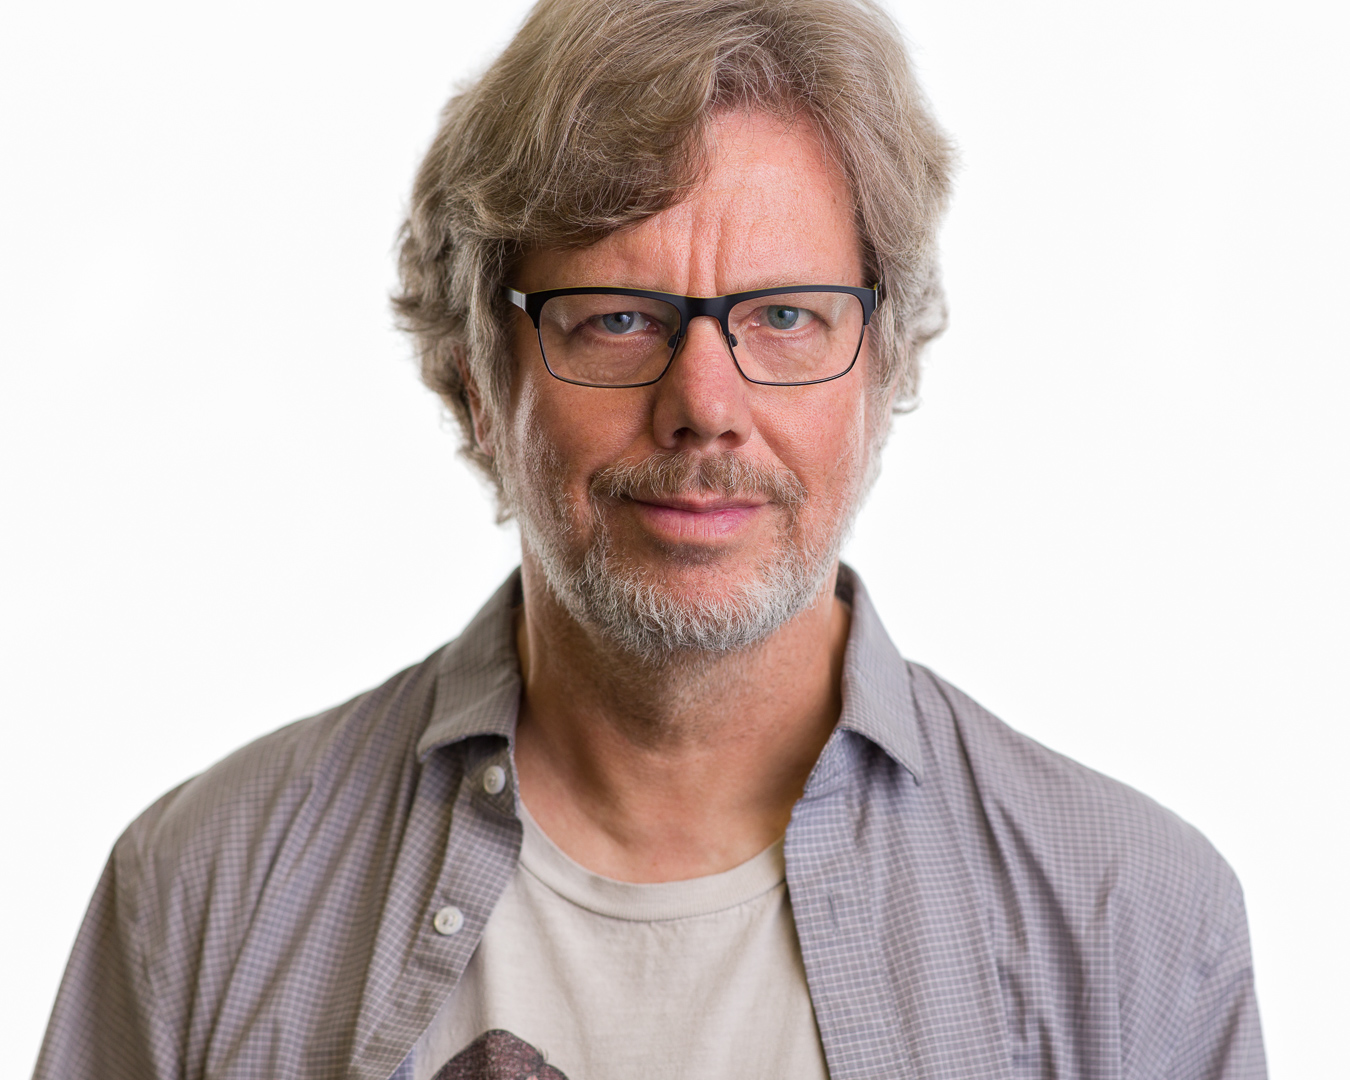
\includegraphics[width=0.25\textwidth]{pictures/guido}
\caption{Гвідо ван Россум}
\label{gvido}
\end{wrapfigure}
Python (Пайтон) — інтерпретована об'єктно-орієнтована мова програмування високого рівня зі строгою динамічною типізацією.  Назву запозичено із назви британського шоу Монті Пайтон. Розроблена в 1990 році Гвідо ван Россумом. 
\end{frame}

\begin{frame}
\frametitle{Версії Python}
%\begin{wrapfigure}{r}{0.35\textwidth}
\begin{figure}
  \begin{center}
    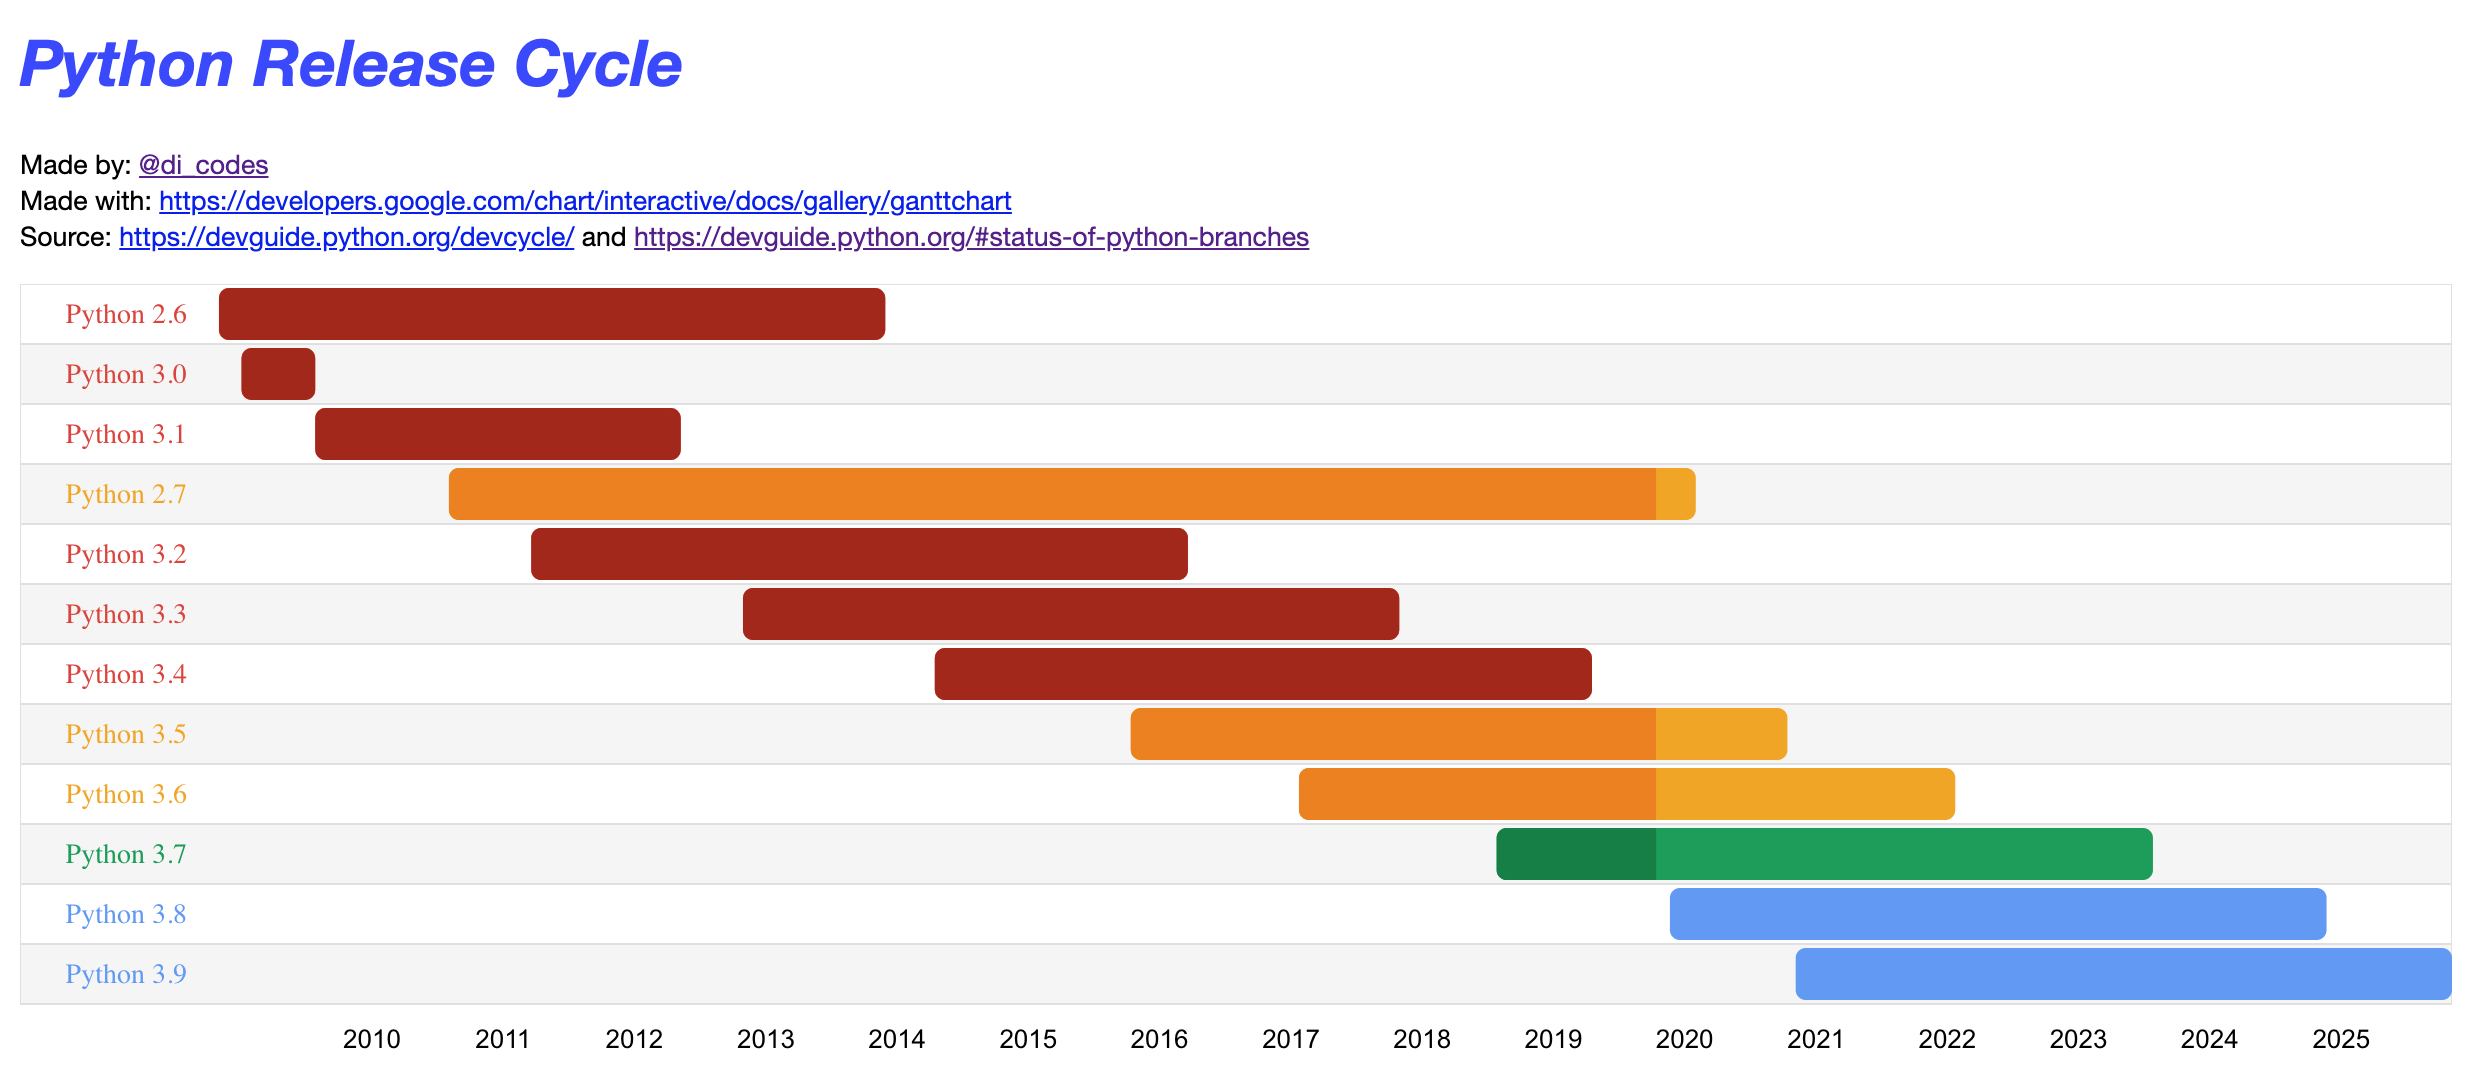
\includegraphics[width=\textwidth,height=0.5\textheight]{pictures/python_versions}
  \caption{Версії Python та період їх підтримки}
\label{versions}
  \end{center}
\end{figure}
\end{frame}

\begin{frame}
\frametitle{Переваги та недоліки Python}
Переваги:
\begin{itemize}
  \item зручність та простота програмування;
  \item переносимість програм;
  \item велика кількість модулів;
  \item поширеність та популярність.
\end{itemize}
Недоліки:
\begin{itemize}
  \item порівняно низька швидкість виконання програм;
  \item неможливість модифікації вбудованих класів.
\end{itemize}
\end{frame}

\begin{frame}
\frametitle{Переваги та недоліки Python}
\begin{itemize}
  \item Python  застосовується при розробці алгоритмів штучного інтелекту (в нейронних мережах);
  \item Python  застосовується при розробці серверної частини сайтів за допомогою Django та Flask (Instagram, YouTube, алгоритми пошуку Google, Dropbox, тощо);
  \item Python  застосовується в наукових проєктах та для обробки даних (Big Data);
  \item Python  застосовується для Web Parsing.
\end{itemize}
\end{frame}


\begin{frame}
\frametitle{Зручність та простота коду Python}
\begin{figure}
\begin{center}
 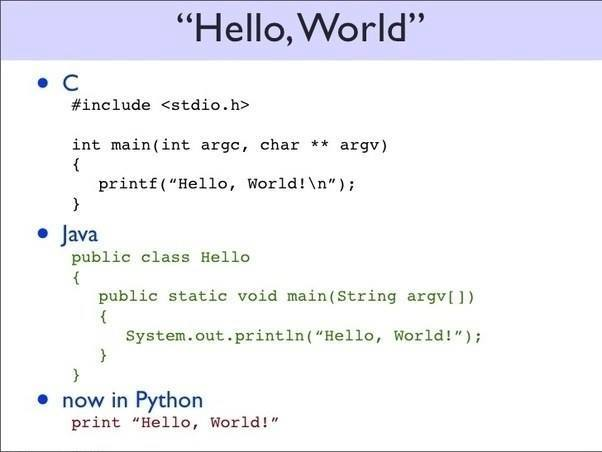
\includegraphics[width=0.4\textwidth]{pictures/helloworld.png}
\caption{Код на C, Java та Python для виведення на екран рядку "Hello, World!"}
\label{python_site} 
\end{center}
\end{figure}
\end{frame}

\begin{frame}
\frametitle{Python має велику кількість бібліотек та фреймворків}
\begin{figure}
\begin{center}
 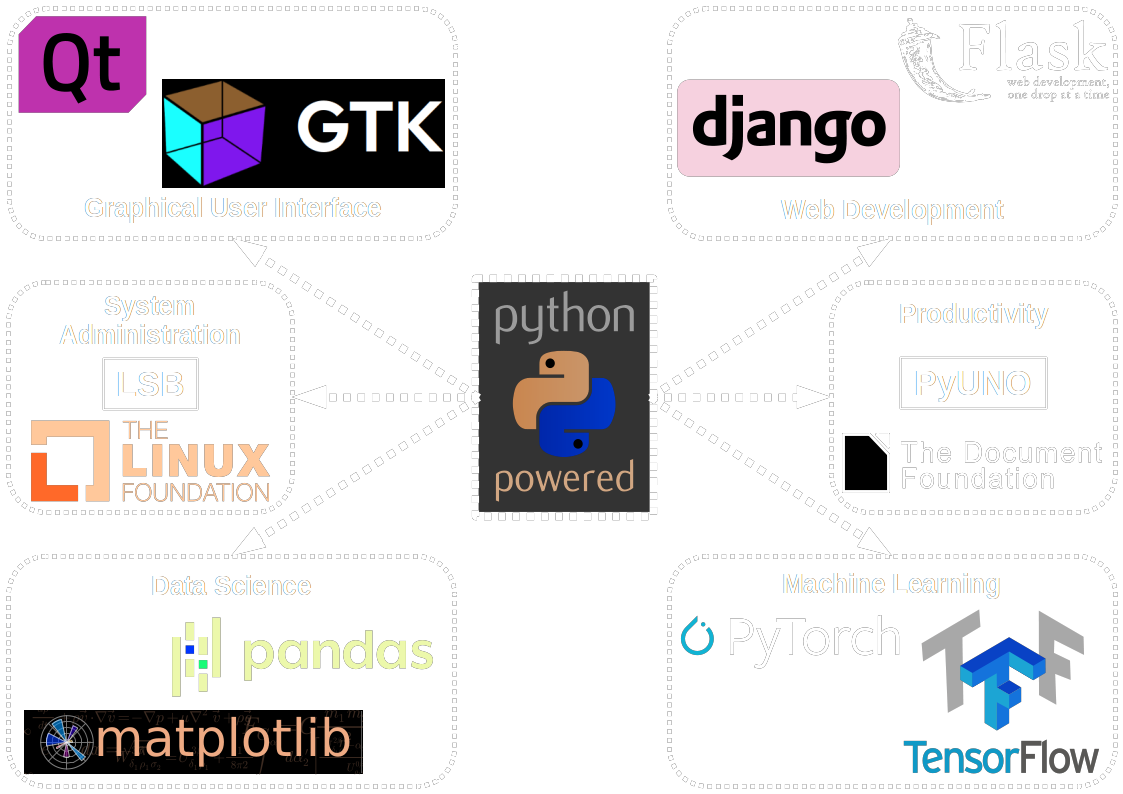
\includegraphics[width=0.6\textwidth]{pictures/python_frameworks1.png}
\caption{Фреймворки Python}
\label{python_site} 
\end{center}
\end{figure}
\end{frame}

\begin{frame}
\frametitle{Python є однією із найпопулярніших мов програмування}
\begin{figure}
\begin{center}
 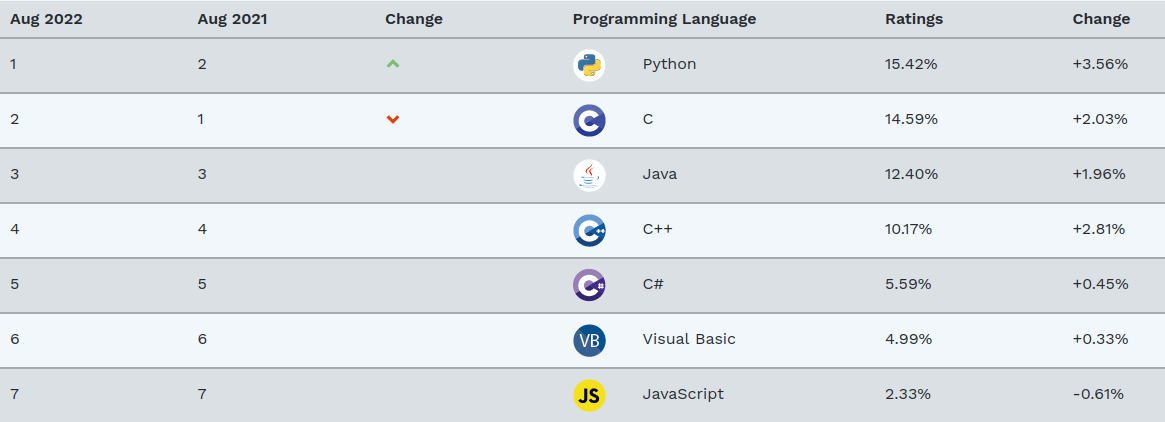
\includegraphics[width=0.6\textwidth]{pictures/tiobe.png}
\caption{З сайту \href{https://www.tiobe.com/tiobe-index/}{TIOBE}}
\label{python_site} 
\end{center}
\end{figure}
\tiny{TIOBE індекс (рейтинг мов програмування) — показник популярності мов програмування. Розраховується виходячи з кількості результів запитів до пошукових систем, що містять назву мови. Охоплює пошуки в Google, MSN, Yahoo!, Baidu, Вікіпедії і Youtube.}
\end{frame}



\subsection{Робота з Python}
\begin{frame}
\frametitle{Сайт Python}
\begin{figure}
\begin{center}
 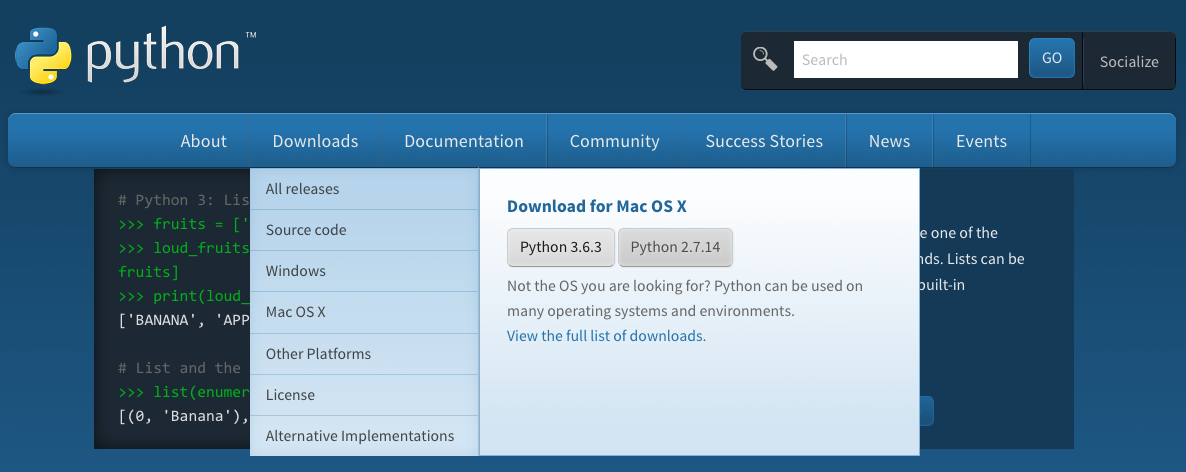
\includegraphics[width=0.95\textwidth]{pictures/python_site.png}
\caption{Сайт: \href{https://python.org/}{python.org}}
\label{python_site} 
\end{center}
\end{figure}

\end{frame}

\begin{frame}
\frametitle{Встановлення Python}
\begin{figure}
\begin{center}
 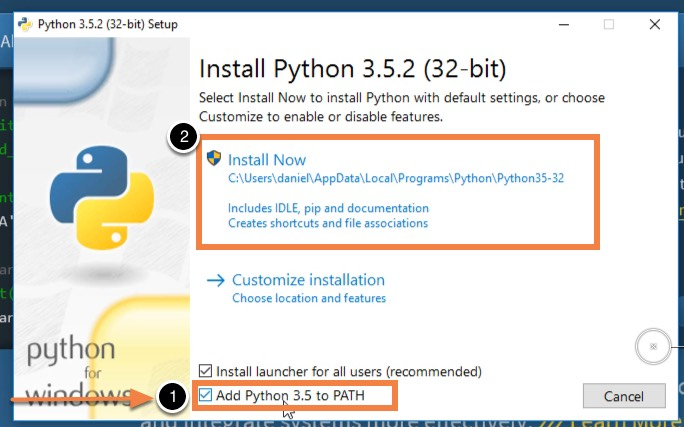
\includegraphics[width=0.4\textwidth]{pictures/python_install.jpg}
\caption{Встановлення Python}
\label{python_install} 
\end{center}
\end{figure}
\tiny{\href{https://uk.wikibooks.org/wiki/}{uk.wikibooks.org/wiki/Пориньте\_у\_Python\_3/Встановлення} - інструкція зі встановлення Python.}
\end{frame}

\begin{frame}
\frametitle{Виконання коду Python}

\begin{wrapfigure}{l}{0.45\textwidth}
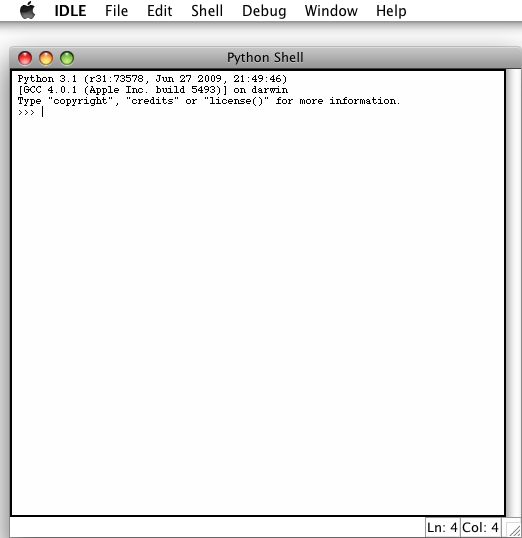
\includegraphics[width=0.35\textwidth]{pictures/idle.png}
\caption{IDLE}
\label{myphoto}
\end{wrapfigure}

Код Python може виконуватися в \textit{інтерактивному} та \textit{файловому} режимі.
\end{frame}


\begin{frame}
\frametitle{Виконання коду Python}
\href{https://it-need.com/pep-8-posibnyk-z-napysannya-kodu-na-python/}{PEP8} містить перелік принципів написання красивого та лаконічного програмного коду мовою Python (PEP – Python Enhancement Proposal, пропозиції щодо розвитку Python).
\begin{figure}
\begin{center}
 
\includegraphics[width=0.5\textwidth]{pictures/pep8.png}
\caption{PEP8}
\label{python_site} 
\end{center}
\end{figure}
\end{frame}

\begin{frame}
\frametitle{PyCharm}


\begin{wrapfigure}{r}{0.4\textwidth}

\includegraphics[width=0.25\textwidth]{pictures/pycharm_logo.png}
\caption{Логотип PyCharm}
\label{pycharm_logo}
\end{wrapfigure}

\textbf{PyCharm} — інтегроване середовище розробки для мови програмування Python. \href{https://www.jetbrains.com/pycharm/download/}{Сайт} для завантаження PyCharm.
\end{frame}


\subsection{Організація курсу}
\begin{frame}
\frametitle{Структура курсу}
\end{frame}

% \section{Лекція 2: Математика в Python}
 
\begin{frame}
\frametitle{Дані в Python}
\begin{itemize}
  \item Змінна - посилання на об'єкт
  \item Оператор присвоювання: 
  
  \texttt{Операнд зліва = Операнд зправа}
  \item Динамічна типізація
  \item \texttt{a = 7; b = a}
  \item Каскадне присвоювання: \texttt{a = b = c = 0}
  \item Множинне присвоювання: \texttt{a, b = 1, 2}
  \item Обмін значеннями: \texttt{a, b = b, a}
\end{itemize}
\end{frame}

\begin{frame}
\frametitle{Функція id}
Функція id(object) повертає «ідентифікаційний номер» об'єкта object, який є унікальним та незмінним.
\begin{figure}
\begin{center}
 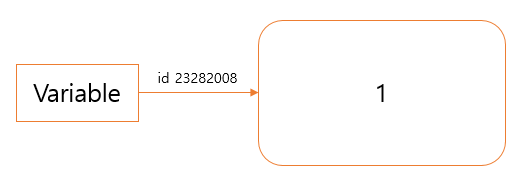
\includegraphics[width=0.7\textwidth]{pictures/id_func.png}
\caption{Функція id}
\label{id} 
\end{center}
\end{figure}
\end{frame}

\begin{frame}
\frametitle{Функція type}
Функция type(object) повертає тип об'єкту object. Його значення таке ж, як у змінної екземпляру object .\_\_ class\_\_.
\begin{figure}
\begin{center}
 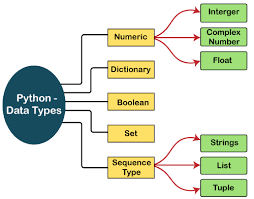
\includegraphics[width=0.5\textwidth]{pictures/python_data_types.png}
\caption{Типи даних в Python}
\label{data_types} 
\end{center}
\end{figure}
\end{frame}


\begin{frame}
\frametitle{Імена змінних}
\begin{itemize}
  \item Перший символ - будь-яка літера латинського алфавіту a-z, A-Z та символ підкреслення \_. Інші символи - теж саме та цифри 0-9.
  \item Іменами слід обирати іменники.
  \item Імена повинні відображати сенс даних.
  \item Неможна використовувати зарезервовані слова (Pycharm - Python Console - help() - keywords).
  \item Не слід використовувати імена вбудованих функцій.
\end{itemize}
\end{frame}
 
\begin{frame}
\frametitle{Типи чисел в Python}
\begin{itemize}
  \item цілі числа (int);
  \item дійсні числа (float);
  \item комплексні числа (complex).
\end{itemize} 
  
\end{frame}

 
\begin{frame}
\frametitle{Арифметичні операції}

\begin{table}
  \caption{Арифметичні операції}
  \label{tab:}

  \begin{center}
    \begin{tabular}{|c|c|c|}
      \hline
      \textbf{Оператор} & \textbf{Опис} & \textbf{Пріоритет} \\
      \hline
      + & додавання & 2 \\
       \hline
      - & віднімання & 2 \\
       \hline
      * & множення & 3 \\
       \hline
       /,// & ділення & 3 \\
       \hline
       \% & залишок від ділення & 3 \\
       \hline
       ** & піднесення в ступінь & 4 \\
       \hline
    \end{tabular}
  \end{center}
\end{table}
 \begin{center}
   \tiny{// - ділення з округленням до найменшого цілого}
  \end{center}
\end{frame}

\begin{frame}
\frametitle{Скорочені оператори в Python}
Оператор += додає значення правого операнда до лівого та присвоює цю суму лівому операнду.

Аналогічно працюють оператори -=, *=, /=, \%=, **=, //=.  
\end{frame}


\begin{frame}
\frametitle{Математичні функції}
\begin{itemize}
  \item abs(a)
  \item min(a, b, ...)
  \item max(a, b, ...)
  \item pow(a, b)
  \item round(a)
  \item round(a, n)
\end{itemize} 
  
\end{frame}

\begin{frame}
\frametitle{Модуль math}
Для того щоб звернутися до функцій модулю math, спочатку треба імпортувати цей модуль командою \texttt{import math}.
\begin{figure}
\begin{center}
 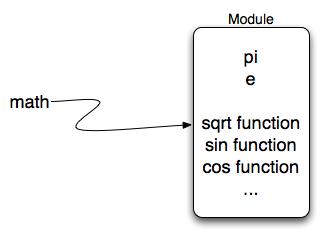
\includegraphics[width=0.5\textwidth]{pictures/mathmod.png}
\caption{Модуль math}
\label{mathmodule} 
\end{center}
\end{figure}
\end{frame}

\begin{frame}
\frametitle{Функції print та input}
\begin{itemize}
  \item print - вивід даних в консоль
      \begin{itemize}
        \item sep - роздільник між даними
        \item end - останній символ (символи)
     \end{itemize} 
  \item input - ввід даних зі стандартного вхідного потоку (клавіатури)
      \begin{itemize}
        \item int(input())
        \item float(input())
     \end{itemize}
 \end{itemize} 
\end{frame}

% \section*{Лекція 3: Рядки}
\subsection{Створення рядків у Python} 
\begin{frame}
\frametitle{Рядки}
Рядок - упорядкований набір символів. Рядок - незмінний тип даних.
\begin{figure}
\begin{center}
 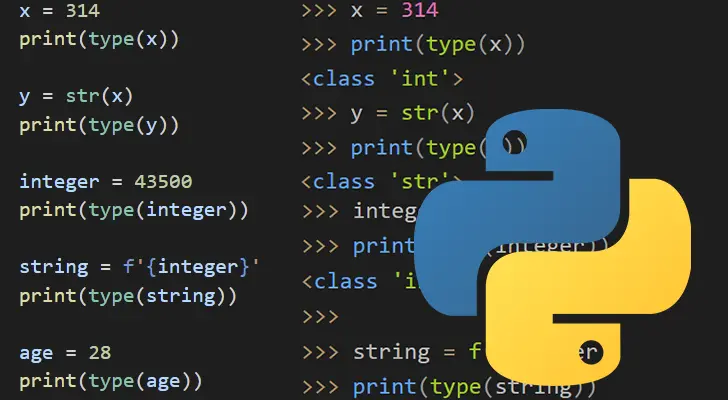
\includegraphics[width=0.6\textwidth]{pictures/strings.png}
\caption{Рядки у Python}
\label{python_site} 
\end{center}
\end{figure}
\end{frame}

\begin{frame}
\frametitle{Створення рядків}
\begin{itemize}
  \item В одинарних лапках 'Python'
  \item В подвійних лапках "Python"
  \item 
  В потрійних лапках '''Python
  
  is the best!'''
  \item Символ переноса рядка \textbackslash n
 \end{itemize}
\begin{figure}
\begin{center}
 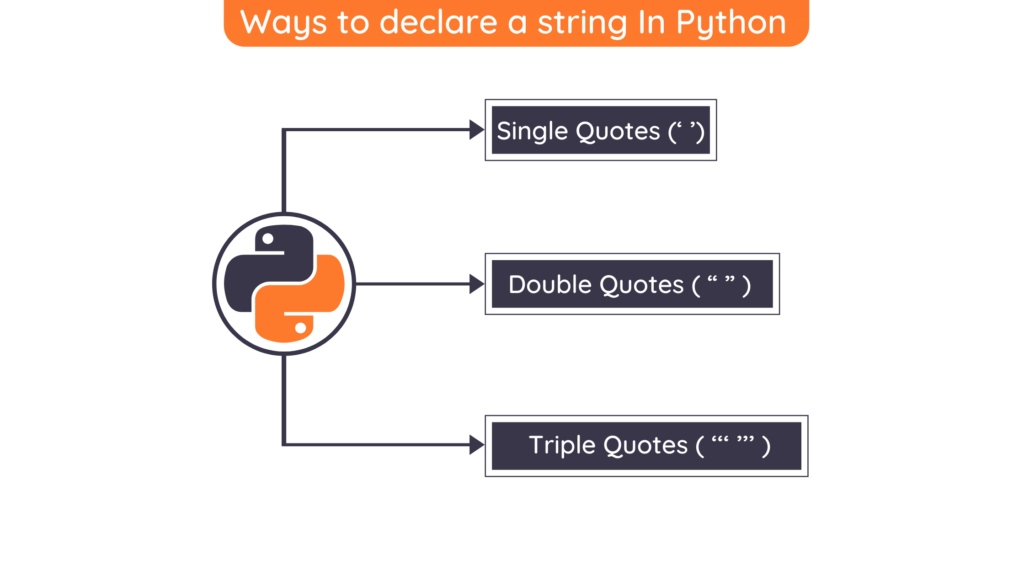
\includegraphics[width=0.4\textwidth]{pictures/declare_string.png}
\caption{Створення рядків у Python}
\label{python_site} 
\end{center}
\end{figure}
\end{frame}

\subsection{Операції над рядками} 
\begin{frame}
\frametitle{Операції над рядками}
\begin{itemize}
  \item Конкатенація рядків (оператор \texttt{+})
  \item Повторення рядків (оператор \texttt{*})
  \item Функція \texttt{str}
  \item Довжина рядка. Функція \texttt{len}
  \item Оператор входження \texttt{in}
 \end{itemize}

\end{frame}

\begin{frame}
\frametitle{Порівняння рядків}
\begin{itemize}
  \item Дорівнює \texttt{==} або не дорівнює \texttt{!=}.
  \item Більше \texttt{>} або менше \texttt{<}.
  \item Функції \texttt{ord} та \texttt{chr}.
\end{itemize}
\begin{figure}
\begin{center}
 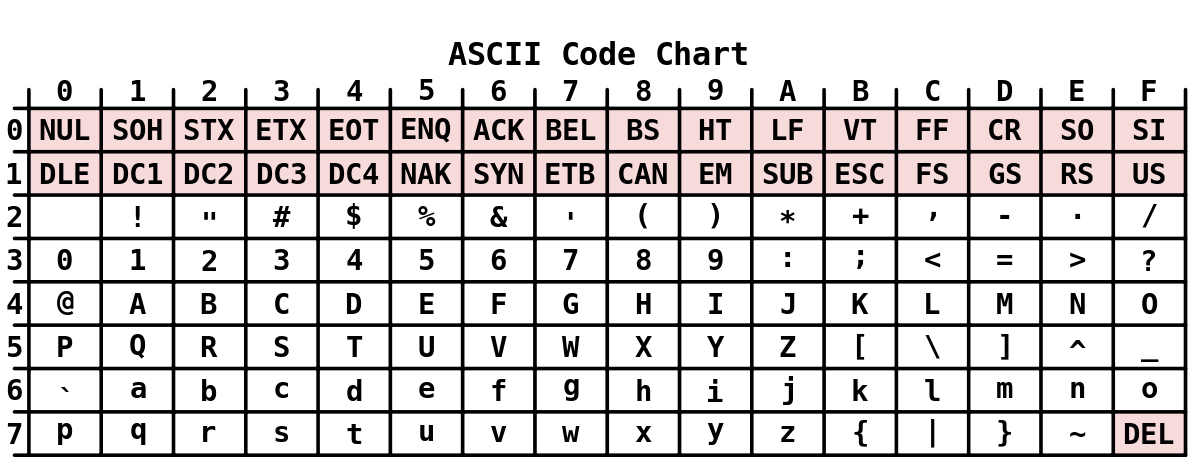
\includegraphics[width=0.7\textwidth]{pictures/ASCII-Table.png}
\caption{Таблиця ASCII}
\label{ASCII-Table} 
\end{center}
\end{figure}
\end{frame}

\begin{frame}
\frametitle{Елементи рядків}
Щоб отримати  i-й елемент рядка s використовується конструкція s[i]. Індекс i змінюється від 0 до len(s) - 1 (або від -1 до -len(s)).
\begin{figure}
\begin{center}
 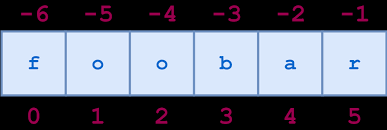
\includegraphics[width=0.5\textwidth]{pictures/string.png}
\caption{Елементи рядка}
\label{string} 
\end{center}
\end{figure}
\end{frame}

\begin{frame}
\frametitle{Зріз рядка}
Зріз (slice) — витяг із рядка одного символу або деякого фрагмента підрядка чи підпослідовності.

\begin{center}
\LARGE{s[start:stop:step]}
\end{center}
\end{frame}

\subsection{Методи рядків} 

\begin{frame}
\frametitle{Методи}
\begin{center}
\texttt{об'єкт.метод(аргументи)}
\end{center}
\begin{figure}
\begin{center}
 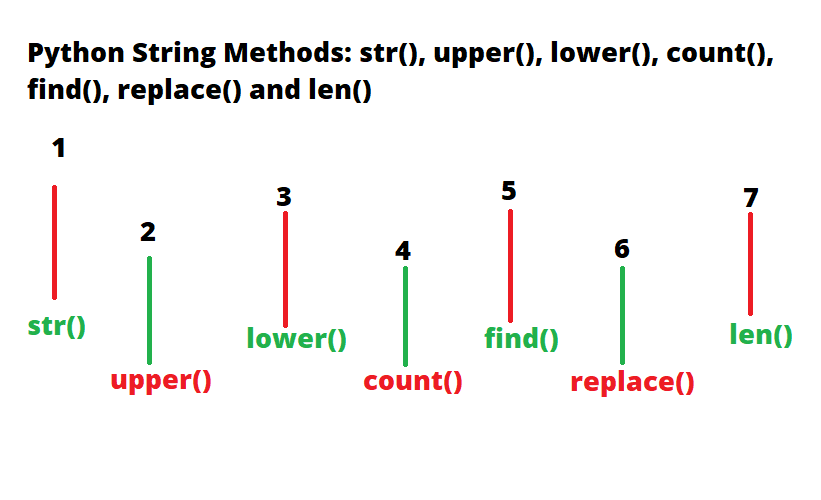
\includegraphics[width=0.5\textwidth]{pictures/python-string-methods.png}
\caption{Методи рядків}
\label{python-string-methods} 
\end{center}
\end{figure}
\end{frame}

\begin{frame}
\frametitle{Методи рядка s}
\begin{itemize}
  \item s.upper() - перетворює всі маленькі літери у великі;
  \item s.lower() - перетворює всі великі літери в маленькі;
  \item s.count(sub[, start[, end]]) - підрахунок кількості підрядків в рядку;
  \item s.find(sub[, start[, end]]) - індекс першого входження підрядка в рядку (find - пошук зліва направо, rfind - пошук зправа наліво);
  \item s.index(sub[, start[, end]]) - аналогічно до find, в разі не знаходження повертає помилку (find повертає -1);
\end{itemize}
\end{frame}

\begin{frame}
\frametitle{Методи рядка s}
\begin{itemize}
 \item s.replace(old, new[, count=-1]) - заміна підрядка old на підрядок new (count - кількість замін, count = -1 - без обмежень);
 \item s.isalpha() - повертає істину якщо рядок повністю складається із літер (інакше -повертає брехню);
 \item s.isdigit() - повертає істину якщо рядок повністю складається із цифр (інакше -повертає брехню);
 \item s.rjust(width[, fillcar=' ']) - повертає рядок заданої ширини width, fillcar - символи, що за потреби додаються зліва (у функції ljust - зправа);
\end{itemize}
\end{frame}

\begin{frame}
\frametitle{Методи рядка s}
\begin{itemize}
 \item s.split(sep=None, maxsplit=-1) - розбиває рядок за вказаним символом sep;
 \item s.join(list) - поєднує елементи списка list через роздільник s;
 \item s.strip(list) - видаляє всі символи пропусків та переносів рядків напочатку та вкінці рядка (rstrip - тільки зліва, lstrip - тільки зправа).
\end{itemize}
\end{frame}

\subsection{Спеціальні символи та методи формування рядків}

\begin{frame}
\frametitle{Спеціальні символи рядків}
\tiny{
\begin{table}
  \caption{Спеціальні символи}
  \label{tab:}

  \begin{center}
    \begin{tabular}{|p{1.2cm}|p{3.5cm}|p{1.2cm}|p{3.5cm}|}
    \hline
     \textbf{Позначення}  & \textbf{Опис} & \textbf{Позначення}  & \textbf{Опис} \\
     \hline
      \textbackslash n & Перевод рядка & \textbackslash \textbackslash & Символ зворотнього слеша \\
     \hline
           \textbackslash ' & Символ апострофа & \textbackslash " & Символ подвійної лапки \\
     \hline
           \textbackslash a & Звуковий сигнал & \textbackslash b & Емуляція клавіші BackSpace \\
     \hline
           \textbackslash f & Переклад формату & \textbackslash r & Повернення каретки \\
     \hline
           \textbackslash t & Горизонтальна табуляція (4 пропуски) & \textbackslash v & Вертикальна табуляція \\
     \hline
           \textbackslash 0 & Символ Null (не признак кінця рядка) & \textbackslash xhh & Символ з шістнадцятковим кодом hh \\
     \hline
           \textbackslash ooo & Символ з вісімковим кодом ooo  & \textbackslash N\{id\} & Ідентифікатор із кодової таблиці Unicode \\
     \hline
           \textbackslash uhhhh & 16-ти бітний символ Unicode в шістнадцятковій формі & \textbackslash Uhhhhhhhh &  32-х бітний символ Unicode в шістнадцятковій формі\\
     \hline
    \end{tabular}
  \end{center}
\end{table}
}
\end{frame}

\begin{frame}
\frametitle{"Сирі" (raw) рядки}
Якщо перед рядком поставити літеру \texttt{r}, то всі символи в ньому будуть сприйматися так, як вони написані.
\begin{figure}
\begin{center}
 
\includegraphics[width=\textwidth]{pictures/raw_string.png}
\caption{Приклад сирого рядка}
\label{raw_string} 
\end{center}
\end{figure}
\end{frame}

\begin{frame}
\frametitle{Методи формування рядків}
name = "Bruce"

age = 35
\begin{itemize}
  \item "My name is " + name + " and my age is " + str(age)
  \item "My name is \{0\} and my age is \{1\}".format(name, age)
  \item "My name is \{fio\} and my age is \{old\}".format(fio=name, old=age)
  \item f"My name is \{name\} and my age is \{age\}"
\end{itemize}
\end{frame}

% \section*{Лекція 4: Списки}
\subsection{Списки та операції над ними} 
\begin{frame}
\frametitle{Створення списків у Python}
Список - впорядкована колекція даних різних типів.

Список відноситься до змінних типів даних.

Пустий список - []. Для створення списку на основі об'єкту, який можна перебирати, використовується функція list.
\begin{figure}
\begin{center}
 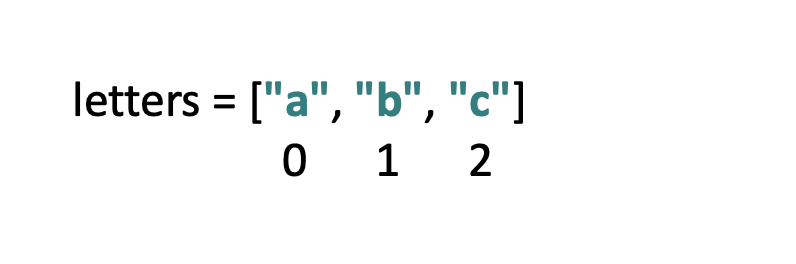
\includegraphics[width=0.6\textwidth]{pictures/list.png}
\caption{Список}
\label{list} 
\end{center}
\end{figure}

\end{frame}

 
\begin{frame}
\frametitle{Основні  функції для роботи зі списком s}
    \begin{itemize}
        \item<1-> \texttt{len(s)} - визначення числа елементів у списку;
        \item<2-> \texttt{max(s)} - знаходження максимального значення;
        \item<2-> \texttt{min(s)} - знаходження мінімального значення;
        \item<3-> \texttt{sum(s)} - розрахунок суми;
        \item<4-> \texttt{sorted(s)} - сортування за зростанням;
        \item<4-> \texttt{sorted(s, reverse=True)} - сортування за спаданням.
    \end{itemize}
\end{frame}

\begin{frame}
\frametitle{Оператори для роботи зі списками}
    \begin{itemize}
        \item<1-> \texttt{+} - поєднання двох списків в один;
        \item<2-> \texttt{*} - повторення списку;
        \item<3-> \texttt{in} - перевірка входження елементу в список;
        \item<4-> \texttt{del} - видалення елементу списку.
    \end{itemize}
\end{frame}

\subsection{Робота зі списками} 
\begin{frame}
\frametitle{Зрізи}
Зрізи дозволяють отримати деяку підмножину значень списку:
\vspace{1cm}
\begin{center}
\huge{lst[start:stop[:step]]}
\end{center}
\normalsize

\end{frame}


\begin{frame}
\frametitle{Копіювання та порівнювання списків}
Для створення копії списка \texttt{lst} використовується команда \texttt{lst[:]} або \texttt{list(lst)}.

Списки можна лексикографічно порівнювати між собою за допомогою операторів: >, <, == та !=.
\begin{table}
  \caption{}
  \label{tab:}

  \begin{center}
    \begin{tabular}{|c|c|}
    \hline
      \textbf{Оператор} & \textbf{Значення} \\
      \hline
      > & більше \\
      \hline
      < & менше\\
      \hline
      == & дорівнює \\
      \hline
      != & не дорівнює\\
      \hline
    \end{tabular}
  \end{center}
\end{table}
\end{frame}

\subsection{Методи списків} 

\begin{frame}
\frametitle{Додаванна та видалення елементів}
\begin{center}
\texttt{об'єкт.метод(аргументи)}
\end{center}
\begin{itemize}
        \item<1-> \texttt{lst.append(el)} - додати елемент el в кінець списку lst;
        \item<2-> \texttt{lst.insert(pos, el)} - додати елемент el до списку lst на місце з індексом pos;
        \item<3-> \texttt{lst.remove(val)} - видаляє перший елемент val зі списку lst (якщо елементу немає в списку, отримуємо помилку);
        \item<4-> \texttt{lst.pop([ind])} - видаляє та \textbf{повертає} останній елемент зі списку lst або елемент з індексом ind.
    \end{itemize}
\end{frame}


\begin{frame}
\frametitle{Аналіз списку}
\begin{center}
об'єкт.метод(аргументи)
\end{center}
\begin{itemize}
        \item<1-> \texttt{lst.clear()} - видаляє всі елементи зі списку lst;
        \item<2-> \texttt{lst.copy()} - повертає копію списку lst;
        \item<3-> \texttt{lst.count(val)} - число елементів зі значенням val в списку lst;
        \item<4-> \texttt{lst.index(val)} - індекс значення val в списку lst;
        \item<4-> \texttt{lst.index(val, start)} - знаходить індекс значення val в списку lst, починаючи з індексу start;
    \end{itemize}
\end{frame}

\begin{frame}
\frametitle{Зміна списку}
\begin{center}
об'єкт.метод(аргументи)
\end{center}
\begin{itemize}
        \item<1-> \texttt{lst.reverse()} - змінює порядок елементів списку lst на зворотній;
        \item<2-> \texttt{lst.sort()} - сортує елементи списку lst за зростанням;
        \item<2-> \texttt{lst.sort(reverse=True)} - сортує елементи списку lst за спаданням;
    \end{itemize}
\end{frame}

\subsection{Додаткові відомості щодо списків} 

\begin{frame}
\frametitle{Вкладені списки} 
\begin{center}
Вкладений список це двовимірний список.

\vspace{1cm}

\Large
lst = [line[:], line[:], line[:]]
\normalsize

\vspace{1cm}

Щоб отримати один елемент використовуємо команду lst[i][j]. 
\end{center}

\end{frame}

\begin{frame}
\frametitle{Сортування} 
Метод \texttt{sort} застосований до списку \texttt{a}: \texttt{a.sort()}  сортує цей список, але нічого не повертає (\texttt{a.sort(reverse=True)} - сортування за убуванням).

Функція \texttt{sorted} застосована до списку \texttt{a}: \texttt{sorted(a)}  повертає відсортований список, але не змінює вихідний (\texttt{sorted(a, reverse=True)} - сортування за убуванням). Функція \texttt{sorted} застосовується до будь-яких ітерованих об'єктів.

\end{frame}

\section*{Лекція 5: Умовні оператори}
 
 \subsection{Логічний тип даних} 
\begin{frame}
\frametitle{True та False}
\begin{itemize}
  \item True - істина
  \item False - брехня
 \end{itemize}

\begin{figure}
\begin{center}
 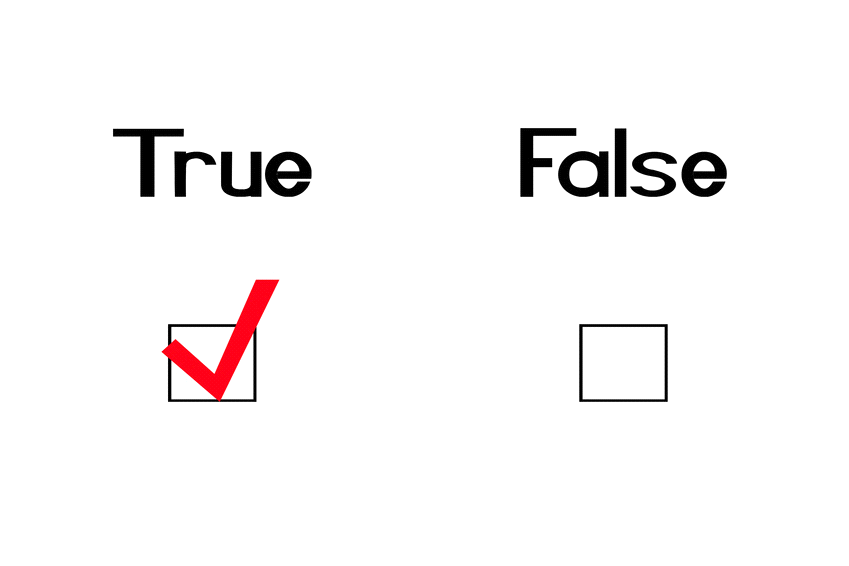
\includegraphics[width=0.4\textwidth]{pictures/TrueFalse.png}
\caption{True або False ?}
\label{TrueFalse} 
\end{center}
\end{figure}
\end{frame}

\begin{frame}
\frametitle{Логічні оператори}

\begin{table}
  \caption{Логічні вирази}
  \label{tab:}

  \begin{center}
    \begin{tabular}{|c|c|}
    \hline
      \textbf{Оператор} & \textbf{Значення} \\
    \hline  
      < & менше \\
    \hline
      >  & більше\\
    \hline
      <=  & менше або дорівнює \\
    \hline
      >=  & більше або дорівнює\\
    \hline
      ==  & дорівнює \\
    \hline
      !=  & не дорівнює \\
    \hline
    \end{tabular}
  \end{center}
\end{table}

\end{frame}

\begin{frame}
\frametitle{Логічні оператори}
\begin{table}
  \caption{Логічні оператори}
  \label{tab:}

  \begin{center}
    \begin{tabular}{|c|c|c|}
    \hline
      \textbf{Оператор} & \textbf{Значення} & \textbf{Пріоритет} \\
    \hline  
      or & або & 1 \\
    \hline
      and & та & 2 \\
    \hline
      not & ні & 3 \\
    \hline
    \end{tabular}
  \end{center}
\end{table}
\end{frame}

\subsection{Типове використання логічних операторів} 
\begin{frame}
\frametitle{Використання логічних операторів}
\begin{itemize}
  \item Перевірка на парність/непарність;
  \item Перевірка на потрапляння/непотрапляння в інтервал;
  \item Функція bool().
 \end{itemize}
\end{frame}

\subsection{Оператор розгалуження} 
\begin{frame}
\frametitle{Оператор if}
if - умовний оператор (оператор розгалуження).

% \begin{center}
\huge{if вираз:

~~~~операції}


\begin{flushleft}
\normalsize
Програма оцінює значення `вираз`, яке може дорівнювати True або False. Програма виконає операції тільки якщо вираз = True. Якщо вираз = False, цей шматок коду не буде виконуватись.
\end{flushleft}
% \end{center}
\end{frame}

\begin{frame}
\frametitle{Оператор if-else}
\Large{if вираз:

~~~~операції 1

else:

~~~~операції 2}


\begin{flushleft}
\normalsize
Операції 1 виконуються тільки якщо вираз істинний (дорівнює True). Якщо вираз дорівнює False, виконуються операції 2. Для розділення цих блоків використовуються відступи.
\end{flushleft}
% \end{center}
\end{frame}


\begin{frame}
\frametitle{Оператор if -elif-else}
\LARGE{if вираз 1:

~~~~операції 1

elif вираз 2:

~~~~операції 2

else:

~~~~операції 3}

\end{frame}

 \subsection{Використання умовного оператору} 
\begin{frame}
\frametitle{Знаходження мінімального}
\begin{figure}
\begin{center}
 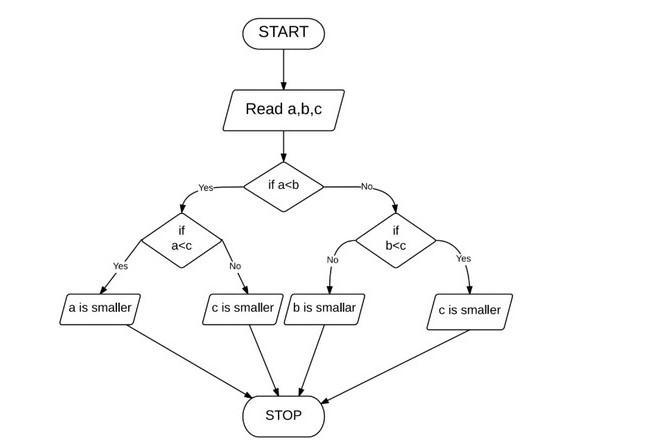
\includegraphics[width=0.4\textwidth]{pictures/find_min.jpg}
\caption{Алгоритм знаходження мінімального із трьох чисел}
\label{find_min} 
\end{center}
\end{figure}
\end{frame}

\begin{frame}
\frametitle{Тернарний умовний оператор}
У Python існує конструкція, яка за своєю дією аналогічна конструкції if-else, але є виразом. Вона називається тернарним оператором.

\Large{\texttt{значення\_1 if умова else значення\_2}}

Тернарний оператор повертає результат.
\end{frame}

\begin{frame}
\frametitle{Функції all та any}
Функція \texttt{all} повертає \texttt{True} якщо всі елементи переданого їй ітерованого об'єкту мають значення \texttt{True}.

Функція \texttt{any} повертає \texttt{True} якщо хоча б один елемент переданого їй ітерованого об'єкту має значення \texttt{True}.
\end{frame}

\subsection{Бітові операції} 
\begin{frame}
\frametitle{Операція НІ}
Бітова операція НІ виконує інверсію біт.

\begin{table}
  \caption{Бітова операція НІ}
  \label{tab:}

  \begin{center}
    \begin{tabular}{|c|c|}
    \hline
      \textbf{х} & \textbf{НІ} \\
    \hline
      0 & 1 \\
    \hline
      1 & 0 \\
    \hline
    \end{tabular}
  \end{center}
\end{table}

В Python бітова операція НІ позначається як $\sim x$.

\end{frame}

\begin{frame}
\frametitle{Операція І}

\begin{table}
  \caption{Бітова операція І: $x_1 \& x_2$}
  \label{tab:}

  \begin{center}
    \begin{tabular}{|c|c|c|}
    \hline
      \textbf{$x_1$} & \textbf{$x_2$} &  \textbf{І} \\
    \hline
      0 & 0 & 0 \\
    \hline
      0 & 1 & 0 \\
    \hline
      1 & 0 & 0 \\
    \hline
      1 & 1 & 1 \\
    \hline
    \end{tabular}
  \end{center}
\end{table}

Можна перевірити чи увімкнено або вимкнути відповідні біти.

\end{frame}

\begin{frame}
\frametitle{Операція АБО}

\begin{table}
  \caption{Бітова операція АБО: $x_1$ | $x_2$}
  \label{tab:}

  \begin{center}
    \begin{tabular}{|c|c|c|}
    \hline
      \textbf{$x_1$} & \textbf{$x_2$} &  \textbf{АБО} \\
    \hline
      0 & 0 & 0 \\
    \hline
      0 & 1 & 1 \\
    \hline
      1 & 0 & 1 \\
    \hline
      1 & 1 & 1 \\
    \hline
    \end{tabular}
  \end{center}
\end{table}

Можна перевірити чи увімкнено або вимкнути відповідні біти.

\end{frame}

\begin{frame}
\frametitle{Операція виключне АБО}

\begin{table}
  \caption{Бітова операція XOR: $x_1 \wedge x_2$}
  \label{tab:}

  \begin{center}
    \begin{tabular}{|c|c|c|}
    \hline
      \textbf{$x_1$} & \textbf{$x_2$} &  \textbf{XOR} \\
    \hline
      0 & 0 & 0 \\
    \hline
      0 & 1 & 1 \\
    \hline
      1 & 0 & 1 \\
    \hline
      1 & 1 & 0 \\
    \hline
    \end{tabular}
  \end{center}
\end{table}

За допомогою XOR можна перемикати біти числа.

\end{frame}

\begin{frame}
\frametitle{Зміщення біт}

\begin{itemize}
  \item $\gg$ - зміщення біт праворуч.
  \item  $\ll$  - зміщення біт ліворуч.

  \item $x = x \gg 1$ - еквівалентно цілочисленному діленню на два.

\end{itemize}


\end{frame}


\end{document}
